\section{Method}\label{method}

Our experiments reveal that quantized LLMs can significantly enhance exploration in RL. Applying parameter-efficient fine-tuning (PEFT) to quantized models not only reduces training resource consumption but also outperforms vanilla LoRA in reward growth and evaluation scores (Fig.\ref{fig:framework}). This challenges the conventional view in SFT that quantization degrades training effectiveness\citep{qlora, guo2023lq}. Notably, we observe that quantization error functions similarly to random noise in networks~\citep{plappert2017parameter, eberhard2023pink,osband2016deep}, promoting broader exploration of potential actions or tokens in RL by increasing entropy (Fig.\ref{fig:entropy_abs}).

% Leveraging the advantage of quantization noise, we propose the QeRL framework, a PEFT training paradigm based on NVFP4. To address the static nature of quantization, we introduce an Adaptive Quantization Noise (AQN) mechanism, which dynamically injects noise during training to enhance the model's exploration capabilities in the reinforcement learning process.


\subsection{Training Framework of QeRL}
QeRL is based on the mainstream policy optimization algorithms of LLMs, such as GRPO~\citep{grpo} and DAPO~\citep{dapo}.

\textbf{Group Relative Policy Optimization}~\citep{grpo} is designed based on the Generalized Advantage Estimation (GAE)~\citep{schulman2015high}, eliminating the need for a separately trained reward model, as required in Proximal Policy Optimization (PPO)~\citep{engstrom2019implementation,schulman2017proximal}. Instead, for a given input query $q$, multiple samples are generated, resulting in a set of candidate outputs $\{o_1, o_2, ..., o_G\}$. These candidates are evaluated using a rule-based reward, and the average reward is used for updates. The optimization objective is defined as follows:
% \begin{equation}\label{eq:grpo}
% \mathcal{J}_{GRPO}(\theta) = \mathbb{E}_{q,\{o_i\}} [ \frac{1}{G} \sum_{i=1}^{G} \frac{1}{|o_i|} \sum_{t=1}^{|o_i|}(\mathrm{min}(\frac{\pi_{\theta}(o_{i,t}|q)}{\pi_{\theta_{old}}(o_{i,t}|q)}A_{i,t}, \mathrm{clip}(\frac{\pi_{\theta}(o_{i,t}|q)}{\pi_{\theta_{old}}(o_{i,t}|q)}, 1-\alpha, 1+\alpha)A_{i,t})  - \beta\mathbb{D}_{KL}(\pi_\theta||\pi_{ref}))]
% \end{equation}
\begin{align}\label{eq:grpo}
\mathcal{J}(\theta) = \mathbb{E}_{q,\{o_i\}} [ \frac{1}{G} \sum_{i=1}^{G} \frac{1}{|o_i|} \sum_{t=1}^{|o_i|}(\mathrm{min}(\frac{\pi_{\theta}(o_{i,t}|q)}{\pi_{\theta_{old}}(o_{i,t}|q)}A_{i,t}, \mathrm{clip}(\frac{\pi_{\theta}(o_{i,t}|q)}{\pi_{\theta_{old}}(o_{i,t}|q)}, 1-\alpha, 1+\alpha)A_{i,t}) \nonumber\\ - \beta\mathbb{D}_{KL}(\pi_\theta||\pi_{ref}))]
\end{align}
% \begin{align}\label{eq:grpo}
% \mathcal{J}_{GRPO}(\theta) = 
% &\; \mathbb{E}_{q,\{o_i\}} \Bigg[ \frac{1}{G} \sum_{i=1}^{G} \frac{1}{|o_i|} \sum_{t=1}^{|o_i|} \Bigg( 
% \mathrm{min}\left(\frac{\pi_{\theta}(o_{i,t}|q)}{\pi_{\theta_{old}}(o_{i,t}|q)}A_{i,t}, \right.\left. \mathrm{clip}\left(\frac{\pi_{\theta}(o_{i,t}|q)}{\pi_{\theta_{old}}(o_{i,t}|q)}, 1-\alpha, 1+\alpha\right)A_{i,t} \right) \Bigg) \nonumber \\
% &\; - \beta\mathbb{D}_{KL}(\pi_\theta||\pi_{ref}) \Bigg]
% \end{align}
where $\pi_{\theta}$ and $\pi_{ref}$ denote the policy model and reference model, respectively, and the clipping range $(1-\alpha, 1+\alpha)$ stabilized the gradient steps of the policy model. KL penalty is used in GRPO to avoid the unexpected large change in updating~\citep{schulman2017proximal}. $A_{i,i}$ is the antagonist of $i^{th}$ completion, shared across all tokens in $o_t$, defined as:
\begin{equation}\label{eq:advantage}
A_i = \frac{r_i - \mathrm{mean}(\{r_1, r_2,...,r_G\})}{\mathrm{std}(\{r_1, r_2,...,r_G\})}
\end{equation}

\textbf{Dynamic Sampling Policy Optimization}~\citep{dapo} suggests higher clipping upper-bond can help avoid entropy collapse. Another improvement in DAPO is to utilize the loss of token-level policy gradients. In DAPO, the KL penalty from Eq.\ref{eq:grpo} is removed to eliminate the upper limit on exploration in RL, thereby encouraging more optional tokens in the rollout process.

% \begin{equation}\label{eq:dapo}
% \mathcal{J}_{DAPO}(\theta) = \mathbb{E}_{q,\{o_i\}} [ \frac{1}{\sum_{i=2}^G |o_i|} \sum_{i=1}^{G}\sum_{t=1}^{|o_i|}(\mathrm{min}(\frac{\pi_{\theta}(o_{i,t}|q)}{\pi_{\theta_{old}}(o_{i,t}|q)}A_{i,t}, \mathrm{clip}(\frac{\pi_{\theta}(o_{i,t}|q)}{\pi_{\theta_{old}}(o_{i,t}|q)}, 1-\alpha_{low}, 1+\alpha_{high})A_{i,t})
% \end{equation}

% \textbf{LoRA Finetuning for Reinforcement Learning}

% To ensure that RL training is not adversely affected by gradient errors in low-bit quantized backpropagation, we adopt the QLoRA~\citep{qlora} structure for mathematic LLMs training. Specifically, the main model is maintained in 4-bit precision (e.g., NVPF4, MXFP4, or NF4) with its parameters frozen, while trainable parameters are integrated through LoRA~\citep{lora}, which incorporates sparse 16-bit trainable parameters. So the update is only for LoRA branch:
% \begin{equation}\label{eq:lora_w}
% \pi_{\theta} \rightarrow \pi_{\theta+\theta_{lora}}, \theta_{lora} \rightarrow \theta_{lora} + \gamma \nabla \mathcal{J}
% \end{equation}


\subsection{Quantization Encourages Exploration}\label{sec:4.2}

To understand how quantization enhances RL, we analyze its effect on the model's sampling behavior. Our central finding is that the noise introduced by quantization serves as an implicit exploration mechanism, similar to explicit noise injection techniques in the parameter and action space~\citep{plappert2017parameter,eberhard2023pink,fortunato2018noisy,liu2025noisyrollout}.

\begin{figure*}[!t]
\begin{center}
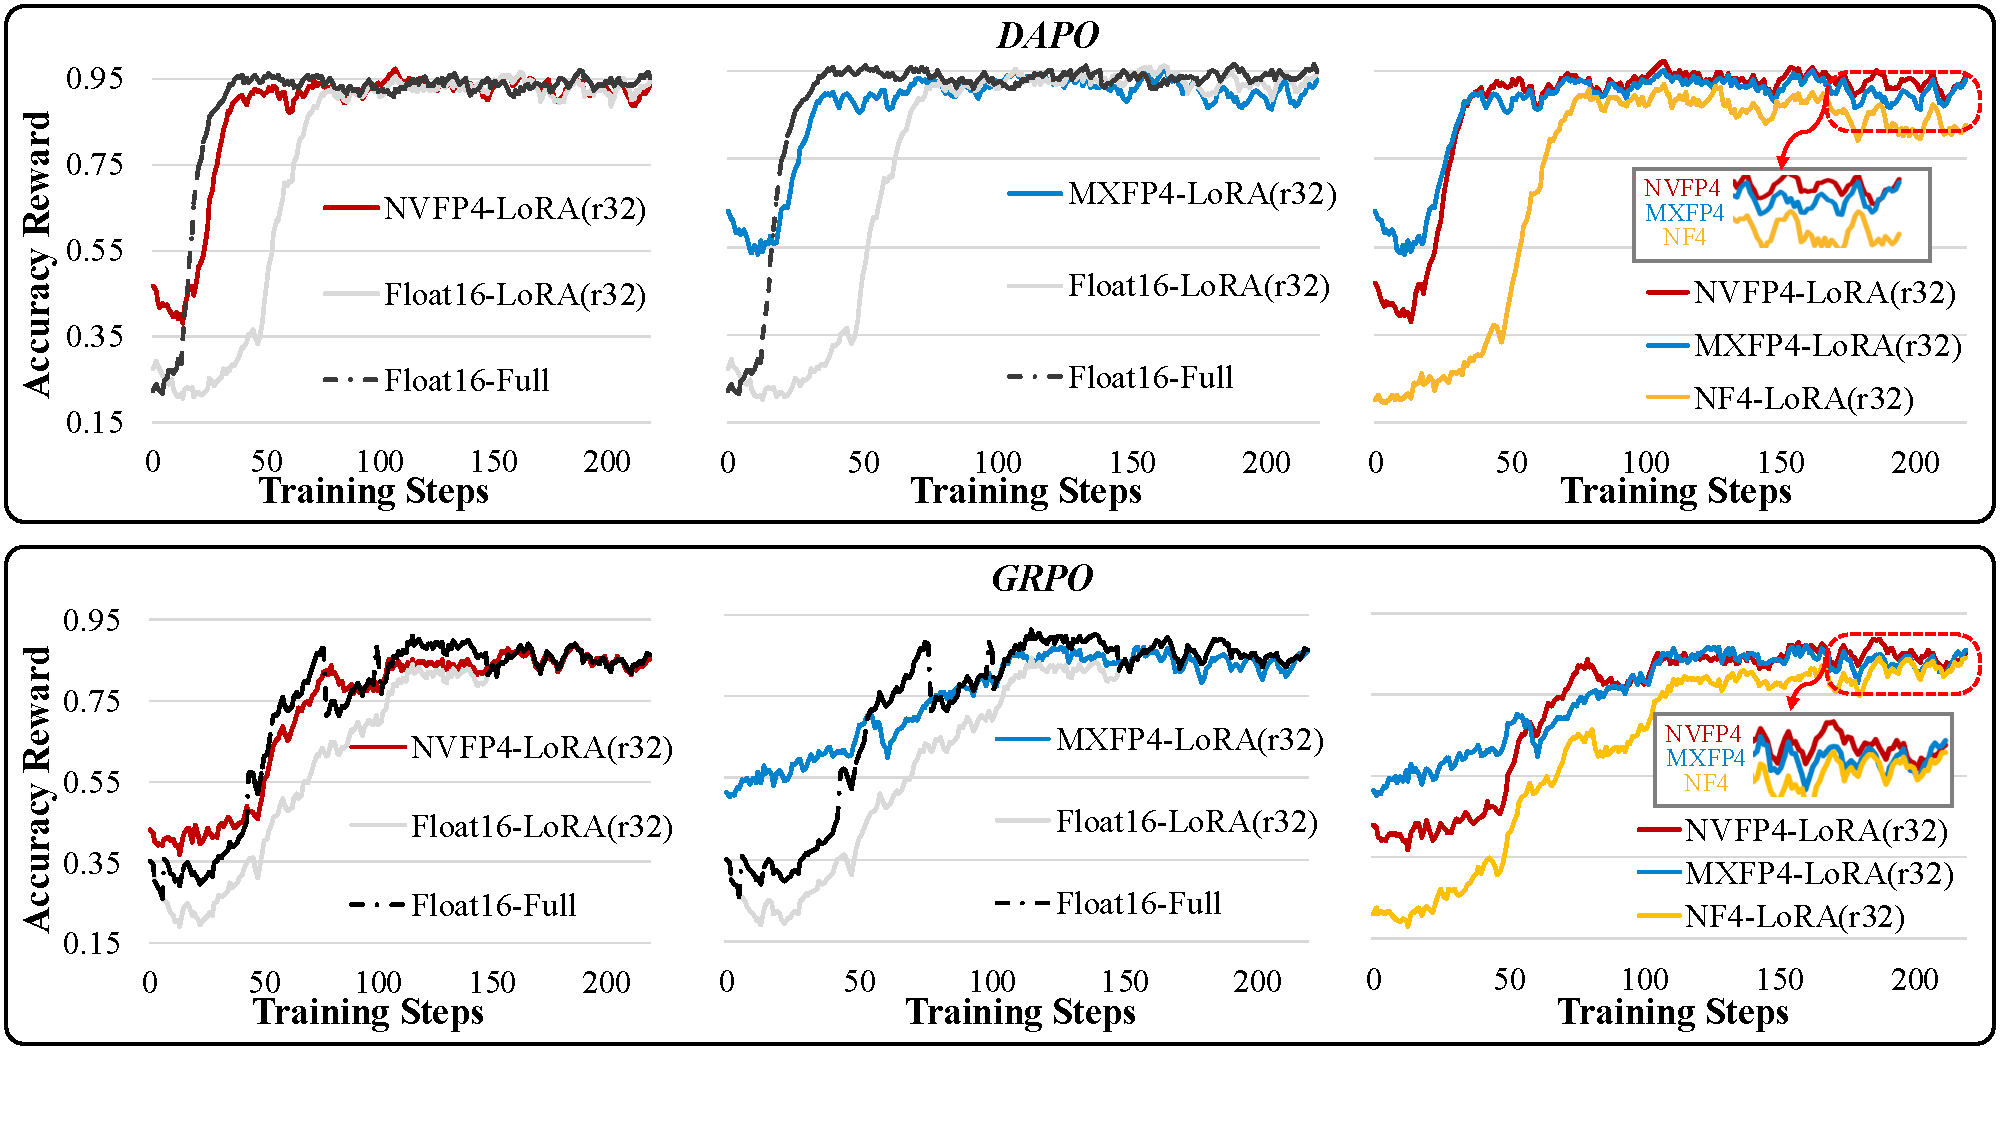
\includegraphics[width=\linewidth]{figures/da_gr_v2.pdf}
\end{center}
\vspace{-0.1in}
\caption{Training reward performance. The upper figures illustrate the training rewards under DAPO, while the lower one is GRPO. Although MXFP4 achieves higher scores in the early stages of training, NVFP4 ultimately converges to better final rewards. LoRA rank is set to 32.}
\label{fig:reward1}
\vspace{-0.1in}
\end{figure*}


\textbf{Quantization Improves Sampling Entropy}
We study 3 different quantization formats of FP4 (NVPF4, MXFP4, and NF4) on GSM8K~\citep{cobbe2021training}.
\begin{wrapfigure}{h}{0.4\textwidth}
%\vspace{-0.3in}
    \centering
    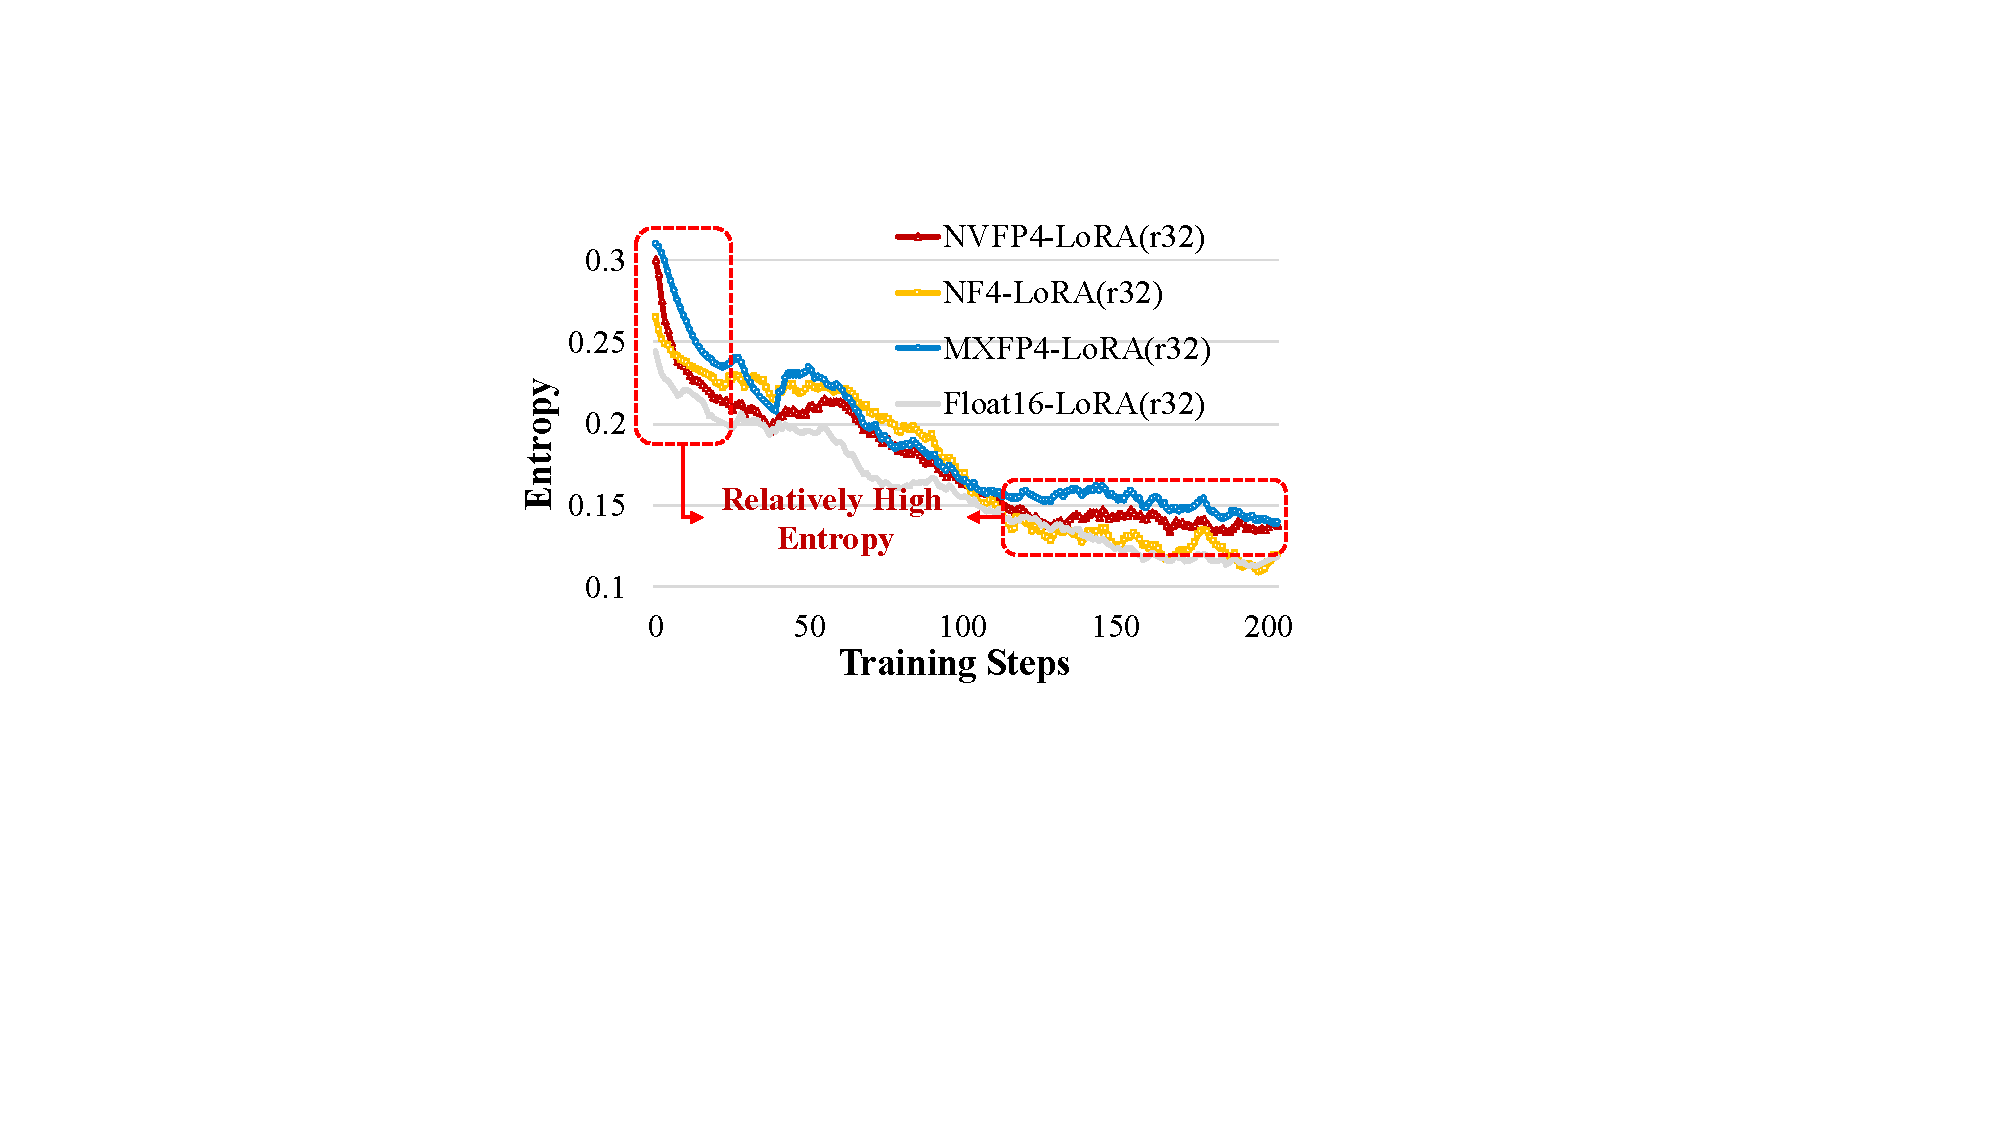
\includegraphics[width=0.4\textwidth]{figures/entropy_v2.pdf} 
    \vspace{-0.2in}
    \caption{
        Comparison of RL entropy. 
    }
    \label{fig:entropy}
\vspace{-0.1in}
\end{wrapfigure}
Our empirical study on Qwen2.5-7B-Instruct~\citep{team2024qwen2} reveals an intriguing finding: when applying PEFT-based RL, models quantized to 4-bit precision consistently outperform their 16-bit counterparts. This advantage is evident across two key metrics: significantly faster reward convergence during training and higher adjusted evaluation scores. As shown in Fig.\ref{fig:reward1}, the reward curves of the models exhibit a steeper upward trend compared to 16-bit models, with convergence patterns closely resembling those of full-parameter fine-tuning in both DAPO and GRPO. Also, NVFP4 and MXFP4 both show better reward growth than NF4.

This unexpected performance improvement prompted us to investigate the underlying mechanism. We discover that quantization inherently increases the sampling entropy, $\mathbf{\mathcal{H}}(\pi(·|q)) = -\sum_{o_t \in V} \pi(o_t|q) \log \pi(o_t|q)$, where $V$ is the vocabulary) of the policy during deployment (shown in Fig.\ref{fig:entropy}). During the forward pass, a quantized model introduces small but systematic errors, which can be modeled as static network noise~\citep{fan2020training}. This noise propagates across the network layers, perturbing the final logits before the softmax function is applied. Consequently, the output probability distribution over the vocabulary, denoted as $\pi_{\theta}(·|q)$, becomes "flatter," with less pronounced peaks. This increase in sampling entropy plays a crucial role in reinforcement learning by encouraging exploration~\citep{cheng2025reasoning,eysenbach2021maximum}. It mitigates the model's overconfidence in a single "optimal" token and instead assigns more meaningful probabilities to a wider range of plausible next actions (Fig.\ref{fig:entropy_abs}). The entropy of other model is provided in Appendix~\ref{ap:more_entropy}.

\textbf{Quantization Noise}
Functionally, this effect resembles exploration in parameters~\citep{eberhard2023pink,plappert2017parameter}, which deliberately injects noise into parameters to drive exploration:
\begin{equation}\label{eq:quantization}
(\mathbf{\tilde{\theta}}+\theta_{lora})-(\mathbf{\theta}+\theta_{lora})=Q(\mathbf{\theta})-\mathbf{\theta}=\Delta\epsilon
\end{equation}
where $Q(\mathbf{\theta})$ denotes the de-quantized weight, and $\Delta\epsilon$ is the quantization noise. Such exploratory noise emerges naturally as a computationally “free” byproduct of compressing model representations. This contrasts starkly with SFT, where noise is often detrimental because the objective is to faithfully imitate the true data distribution rather than to discover novel high‑reward outputs.

% Quantization Noisy in parameter space DAPO:
% \begin{equation}\label{eq:quantization}
% (\mathbf{\tilde{\theta}}+\theta_{lora})-(\mathbf{\theta}+\theta_{lora})=Q(\mathbf{\theta})-\mathbf{\theta}=\Delta\epsilon
% \end{equation}

% Let the pre-trained model be denoted by $\pi_{\theta}$. We first obtain a quantized and frozen base model $\pi_{\tilde{\theta}}$, where $\tilde{\mathbf{\theta}} = Q(\mathbf{\theta})$. The model is then augmented with a set of trainable low-rank adapters, parameterized by $\theta_{lora}$. The effective parameters used during the forward pass are a dynamic combination of the quantized base and the adapter's output, $\mathbf{\tilde{\theta}}+\theta_{lora}$, and we get $\pi_{\theta+\theta_{lora}} \rightarrow \pi_{\theta+\theta_{lora}+\Delta\epsilon}$. 

% \begin{equation}\label{eq:grpo_noise}
% \mathcal{J}(\theta)=\mathbb{E}_{q,\{o_i\}} [ \frac{1}{\sum_{i=2}^G |o_i|} \sum_{i=1}^{G}\sum_{t=1}^{|o_i|} (\mathrm{min}(\frac{\pi_{\mathbf{\theta}+\theta_{lora}+\Delta\epsilon}(o_{i,t}|q)}{\pi_{\theta_{old+\theta_{lora}+\Delta\epsilon}}(o_{i,t}|q)}A_{i,t}, \mathrm{clip}(\frac{\pi_{\mathbf{\theta}+\theta_{lora}+\Delta\epsilon}(o_{i,t}|q)}{\pi_{\theta_{old+\theta_{lora}+\Delta\epsilon}}(o_{i,t}|q)}, 1-\alpha, 1+\alpha)A_{i,t})]
% \end{equation}

% Gradient:
% \begin{equation}\label{eq:frpo_gradient}
% \nabla_{\theta_{lora}} \mathcal{J}_{GRPO} = \mathbb{E} [\frac{1}{G}\sum_{i=1}^{G} \nabla_{\theta_{lora}} log \pi(o_i|q;\mathbf{\theta},\theta_{lora},\Delta\epsilon) \cdot A_i^G] - \beta \nabla_{\theta_{lora}} D_{KL}
% \end{equation}
A key limitation of quantization errors is their deterministic nature, which fails to align with the dynamic exploration-exploitation trade-off required in RL. Unlike stochastic noise in traditional RL~\citep{plappert2017parameter,osband2016deep}, which is randomly sampled and independently applied at different training stages, quantization noise remains static throughout the process, lacking the adaptability needed to enhance exploration at critical phases.


\subsection{Adaptive Quantization Noise in Parameter Space}

To transform static quantization noise into a dynamic exploration mechanism, we introduce an \textit{Adaptive Quantization Noise} (AQN) technique. The core idea is to introduce a small set of structured modulation vectors that slightly perturb the otherwise static quantization noise. In our approach, we utilize an advanced quantization format, NVFP4.

\textbf{NVFP4 Quantization} NVFP4 represents weights using a dual-scaling mechanism: a coarse, per-tensor global scaling factor in FP32, $S_{\text{FP32}}$, and a fine-grained tensor of block-wise FP8 (E4M3) scalers, $\mathbf{S}_{\text{E4M3}}$. The dequantization of a 4-bit $\tilde{\mathbf{W}}$ to the high-precision $\hat{\mathbf{W}}$ follows:
\begin{equation}\label{eq:nvfp4_dequant}
\hat{\mathbf{W}} = \operatorname{Dequant}(\tilde{\mathbf{W}}) = S_{\text{FP32}} \cdot (S_{\text{E4M3}} \odot \tilde{\mathbf{W}})
\end{equation}
where $\odot$ denotes block-wise scalar multiplication, broadcasting each scaler in $S_{\text{E4M3}}$ to its corresponding block of 4-bit weights in $\tilde{\mathbf{W}}$. The quantization noise of each weight matrix, $\Delta\epsilon= \hat{\mathbf{W}} - \mathbf{W}$, is the difference between this reconstructed tensor and the original full-precision tensor $\mathbf{W}$.


\textbf{Adaptive Quantization Noise} We introduce a noise vector to the static quantized weight. Specifically, for each quantized linear layer, we sample a stochastic noise vector, $\mathbf{Z}_{\text{noisy}} \in \mathbb{R}^{1\times d}$, where $d$ is the input dimension of the layer. This vector is not fixed but is resampled for each forward pass. We define it as: $\mathbf{Z}_{\text{noisy}} =\boldsymbol{\epsilon}, \boldsymbol{\epsilon} \sim \mathcal{N}(0, \sigma^2I)$, where $\sigma$ is a hyperparameter in different training stage governing the noise scale, and $\boldsymbol{\epsilon}$ is a random vector whose elements are drawn independently from a standard Gaussian distribution~\citep{plappert2017parameter}. Then the additive noise is defined as:
\begin{equation}\label{eq:dequant_fp_learn}
\Delta\epsilon'= \mathbf{Z}_{\text{noisy}}  + \Delta\epsilon= \mathbf{Z}_{\text{noisy}}  +  \left(\hat{\mathbf{W}} - \mathbf{W}\right)
\end{equation}
where $\Delta\epsilon'$ is equivalent to the dynamic noise of each weight matrix. In our setting, we freeze the main branch weight and update the low-rank matrix during RL. The $\mathbf{W}$ and $\hat{\mathbf{W}}$ are consistent values. In the early stages, we leverage the inherent quantization noise to enhance the model's exploration capabilities. As training progresses, $\sigma$ gradually reduces following an exponential decay scheduler:
\begin{equation}\label{eq:sigma_decy}
\sigma(k) = \sigma_{\text{start}} \cdot \left( \frac{\sigma_{\text{end}}}{\sigma_{\text{start}}} \right)^{\frac{k - 1}{K - 1}}
\end{equation}
where $\sigma_{\text{start}}$ and $\sigma_{\text{end}}$ represent the initial and final noise levels, $k$ is the current stage, and $K$ is the total interval, which are evenly divided in the training steps (more scheduler comparison in Sec.\ref{sec:ablation_decay}). For instance, our experiments in GSM8K with a total of around 600 training steps, noise is injected at 10 evenly spaced intervals, initialized with quantization noise, then from $\sigma_{\text{start}}$ to $\sigma_{\text{end}}$. This approach aims to balance exploration and exploitation~\citep{fox2015taming}.

\begin{wrapfigure}{t}{0.5\textwidth}
\vspace{-0.2in}
    \centering
    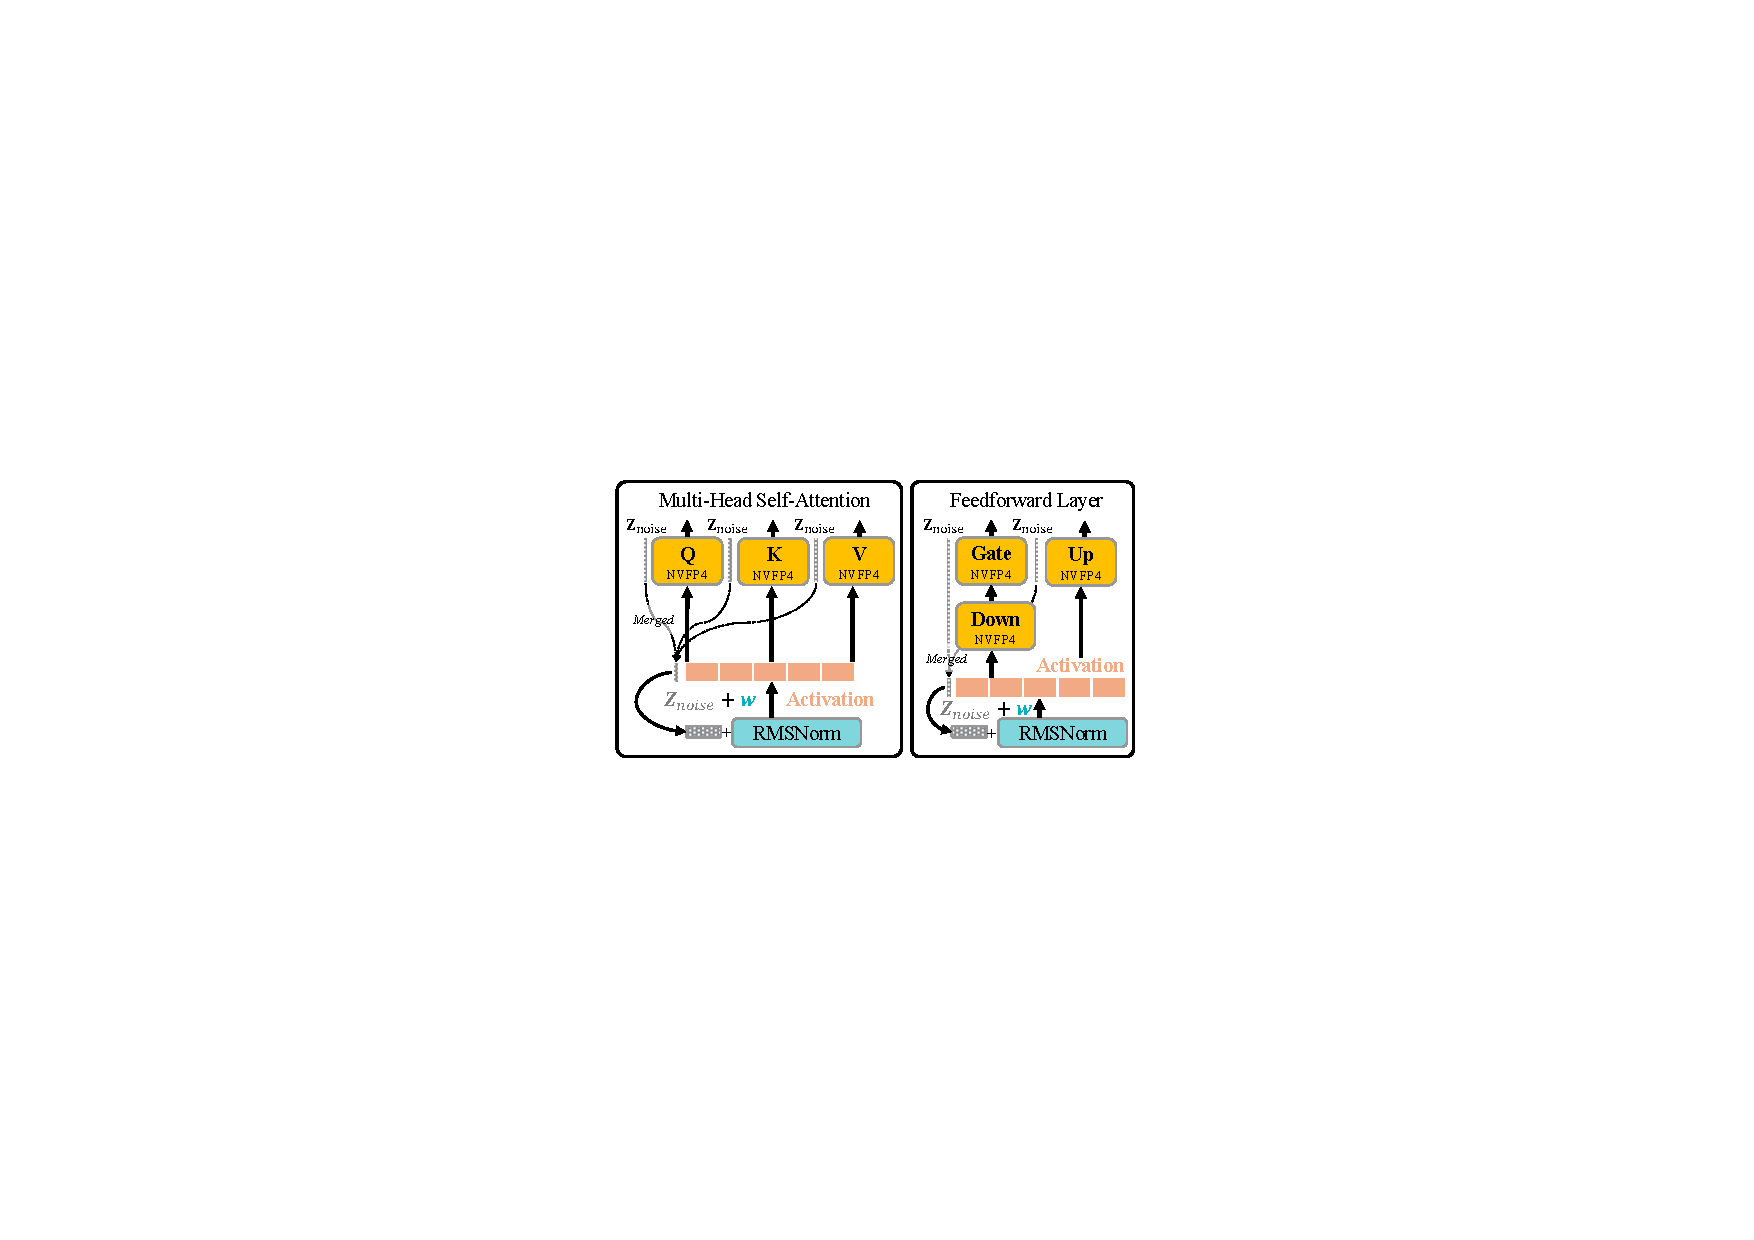
\includegraphics[width=0.5\textwidth]{figures/noise_merge.pdf} 
    %\vspace{-0.1in}
    \caption{
        Deployment scheme of adaptive quantization noise in LLMs. $\mathbf{Z}_{noise}$ is integrated in \textit{LayerNorm} (e.g., RMSNorm) of each block in LLMs.
    }
    \label{fig:dqn}
\vspace{-0.2in}
\end{wrapfigure}
\textbf{Noise Merging} While introducing a noise vector enables dynamic control over quantization noise, explicitly creating a separate vector for each quantized layer is not feasible. First, it imposes a burden on parameter efficiency, increasing memory overhead. Moreover, high-precision noise cannot be directly added to quantized weights, as this would break the compatibility of our inference kernel designed for NVFP4 $\times$ BF16 operations. We propose a simple solution that integrates this noise vector directly into the layer normalization parameters of LLM architectures.

\begin{equation}\label{eq:noise_mul}
    \mathbf{X} \left(\mathbf{Z}_{\text{noisy}} + \hat{\mathbf{W}}\right) =  \mathbf{X} \cdot \mathbf{Z}_{\text{noisy}} + \mathbf{X}\cdot\hat{\mathbf{W}}
\end{equation}
By exploiting this equivalency in Eq.\ref{eq:noise_mul}, we subsume the role of $\mathbf{Z}_{\text{noisy}}$ into the learnable weight parameter of the LayerNorm operation (e.g. RMSNorm~\citep{zhang2019root}) that typically follows the scaling after normalization. 
\begin{equation}\label{eq:sharing}
    \operatorname{RMSNorm}_{noise}(\mathbf{x}) = \mathbf{w}_{noise} \odot \frac{\mathbf{x}}{\sqrt{\frac{1}{N} \sum^N_{i=1}x_i^2+\delta}}, \mathbf{w}_{noise} = \mathbf{Z}_{noise} + \mathbf{w}
\end{equation}
where $\mathbf{w}$ represents the scaling factor of RMSNorm. In this configuration, channel-wise additive noise $\mathbf{Z}_{\text{noisy}}$ transfers to row-wise multiplicative noise $\frac{\mathbf{Z}_{noise}}{\mathbf{w}} +  I$ of weight (proof provided in Appendix~\ref{ap:proof}). Multiplicative noise has been shown to be effective in RL~\citep{pang2021robust,zhang2025reinforcement}. Due to the higher sensitivity of RL to multiplicative noise, we initialize the noise level with $\sigma_{\text{start}} = 1\text{e-}2$ to ensure stability.


This approach extends adaptive quantization noise to the layer parameters $\mathbf{W}_q$, $\mathbf{W}_k$, $\mathbf{W}_v$, $\mathbf{W}_{\text{gate}}$, and $\mathbf{W}_{\text{up}}$ within each block, as these layers directly interact with normalized activations. To align with LLM architectures~\citep{team2024qwen2,grattafiori2024llama}, $\mathbf{W}_q$, $\mathbf{W}_k$, and $\mathbf{W}_v$ share the same RMSNorm, while $\mathbf{W}_{\text{gate}}$ and $\mathbf{W}_{\text{up}}$ share another (as shown in Fig.\ref{fig:dqn}). 
% By fine-tuning $\mathbf{w}$ alongside this approach, the method simplifies training and proves particularly effective for PEFT of LLMs in RL.

% To implement this, $\mathbf{S}_{def}$ can either be manually assigned specific values, similar to the approach in [3] (manually assigned noisy network), or initialized as an identity vector (all ones) with $\mathbf{w}$ set as trainable, resembling the approach in [2] (learnable noisy network). In the latter case, $\mathbf{S}_{def}$ is effectively embedded into $\mathbf{w}$, allowing the RMSNorm layer to implicitly learn the corrective scaling originally intended for $\mathbf{S}_{def}$. In our experiments, we adopt the second approach by initializing $\mathbf{S}_{def}$ as an identity vector and making $\mathbf{w}$ trainable. During RL, we fine-tune only the gradients of $\mathbf{w}$, allowing the RMSNorm layer to automatically learn the scaling originally intended for $\mathbf{S}_{\text{def}}$. 

% In this approach, we specifically apply the deformable quantization noise to $\mathbf{W}_q, \mathbf{W}_k, \mathbf{W}_v$, $\mathbf{W}_{gate}$ and $\mathbf{W}_{up}$ within each block, as these layers directly interact with normalized activations. To ensure consistency with LLM architecture, $\mathbf{W}_q, \mathbf{W}_k, \mathbf{W}_v$ share the same $\operatorname{RMSNorm}$, while $\mathbf{W}_{gate}$ and $\mathbf{W}_{up}$ are also assigned a shared $\operatorname{RMSNorm}$.

% This integration offers several critical advantages. First, it introduces zero overhead because no additional parameters are added. Second, it enables channel-wise control since the dimensions of the RMSNorm weight tensor naturally align with the hidden size, allowing precise feature-specific adjustments. Finally, it ensures smooth and stable training by embedding the scaling factor within a well-established and robust RMSNorm layer. This avoids potential instabilities from introducing new scaling factors and leverages the mature optimization properties of existing components. Effectively, this approach simplifies the training process by requiring only the fine-tuning of $\mathbf{w}_{norm}$ which seamlessly adapts to learn the necessary scaling over the course of training. This method achieves efficient adaptation with negligible computational and memory overhead, making it particularly suitable for parameter-efficient fine-tuning of large language models.







